\documentclass{article}
\setlength{\headheight}{36pt}
\addtolength{\topmargin}{-24pt}
\usepackage{indentfirst}
\usepackage{fancyhdr}
\usepackage{amsmath}
\usepackage{amssymb}
\usepackage{graphicx}
\usepackage[margin=1in]{geometry}
\usepackage{hyperref}
\usepackage[T1]{fontenc}
\usepackage[utf8]{inputenc}
\usepackage{xcolor}
\usepackage{listings}
\usepackage{listingsutf8}
\usepackage[portuguese]{babel}
\usepackage{textcomp}

\title{Resolução da Lista de Exercícios}
\author{\textbf{Francisco Davi Belo Rodrigues}}
\date{\today}

\begin{document}

\fancyhead{}
\fancyhead[C]{%
  {\large\textbf{Universidade Federal do Rio de Janeiro}}\\
  {\normalsize Programa de Pós-Graduação em Engenharia de Processos Químicos e Bioquímicos} \\
  {\normalsize Disciplina EQE 776 - Modelagem e Simulação de Processos}
}

\maketitle
\thispagestyle{fancy}

\section{Exercício 1}

\subsection*{Enunciado e dados}
Consideram-se dois tanques cilíndricos interligados em série. O tanque 1 recebe uma alimentação constante e descarrega no tanque 2, que por sua vez escoa para o ambiente. As vazões de saída de cada tanque dependem do nível interno segundo a relação empírica $Q_i = k_i\sqrt{h_i}$. Os parâmetros fornecidos são resumidos na Tabela~\ref{tab:dados-q1}.

\begin{table}[h!]
  \centering
  \begin{tabular}{ll}
    \hline
    \textbf{Parâmetro} & \textbf{Valor} \\
    \hline
    Vazão de alimentação $Q_0$ & $20\ \mathrm{m^3\,h^{-1}}$ \\
    Diâmetro do tanque 1 $D_1$ & $4\ \mathrm{m}$ \\
    Diâmetro do tanque 2 $D_2$ & $3\ \mathrm{m}$ \\
    Constante da válvula 1 $k_1$ & $14\ \mathrm{m^{2.5}\,h^{-1}}$ \\
    Constante da válvula 2 $k_2$ & $12\ \mathrm{m^{2.5}\,h^{-1}}$ \\
    Nível inicial no tanque 1 $h_1(0)$ & $3\ \mathrm{m}$ \\
    Nível inicial no tanque 2 $h_2(0)$ & $2\ \mathrm{m}$ \\
    \hline
  \end{tabular}
  \caption{Dados operacionais da Questão 1.}
  \label{tab:dados-q1}
\end{table}

\subsection*{Formulação do modelo}

a) \textbf{Construção das equações de balanço}
\begin{enumerate}
  \item A área transversal de cada tanque é $A_i = \pi D_i^2 / 4$, resultando em $A_1 = 12{,}566\ \mathrm{m^2}$ e $A_2 = 7{,}069\ \mathrm{m^2}$.
  \item A conservação de volume líquido em cada tanque fornece
  \begin{align}
    A_1 \frac{dh_1}{dt} &= Q_0 - Q_1, \\
    A_2 \frac{dh_2}{dt} &= Q_1 - Q_2.
  \end{align}
  \item Substituindo a lei das válvulas, obtém-se o sistema não linear
  \begin{align}
    \frac{dh_1}{dt} &= \frac{Q_0 - k_1\sqrt{h_1}}{A_1}, \\
    \frac{dh_2}{dt} &= \frac{k_1\sqrt{h_1} - k_2\sqrt{h_2}}{A_2}.
  \end{align}
\end{enumerate}

b) \textbf{Consistência de unidades}
\begin{enumerate}
  \item Convertem-se as vazões de $\mathrm{m^3\,h^{-1}}$ para $\mathrm{m^3\,s^{-1}}$: $Q_0^{(s)} = Q_0/3600 = 5{,}556 \times 10^{-3}\ \mathrm{m^3\,s^{-1}}$.
  \item As constantes de válvula são tratadas como $k_i^{(s)} = k_i/3600$, de forma que $Q_i = k_i^{(s)}\sqrt{h_i}$ em segundos.
  \item As equações finais utilizadas na simulação tornam-se
  \begin{align}
    \frac{dh_1}{dt} &= \frac{Q_0^{(s)} - k_1^{(s)}\sqrt{h_1}}{A_1}, \\
    \frac{dh_2}{dt} &= \frac{k_1^{(s)}\sqrt{h_1} - k_2^{(s)}\sqrt{h_2}}{A_2},
  \end{align}
  com $h_1(0)=3\ \mathrm{m}$ e $h_2(0)=2\ \mathrm{m}$.
\end{enumerate}

\subsection*{Resolução numérica}
O sistema diferencial foi integrado em $0 \leq t \leq 20\ \mathrm{h}$ (equivalente a $72\,000\ \mathrm{s}$) empregando o método Runge--Kutta de quarta/quinta ordem adaptativo (\texttt{solve\_ivp} do SciPy) com passo máximo de $10\ \mathrm{s}$. A implementação registra também as trajetórias discretizadas $(t, h_1, h_2)$ em arquivo auxiliar para rastreabilidade.

\subsection*{Resultados}
As curvas temporais obtidas para os níveis de líquido encontram-se na Figura~\ref{fig:questao1}. Observa-se que $h_1$ decai de $3\ \mathrm{m}$ para $2{,}04\ \mathrm{m}$, enquanto $h_2$ aumenta para $2{,}78\ \mathrm{m}$ ao final das 20 horas de operação, aproximando-se de um estado quase estacionário.

\begin{figure}[h!]
  \centering
  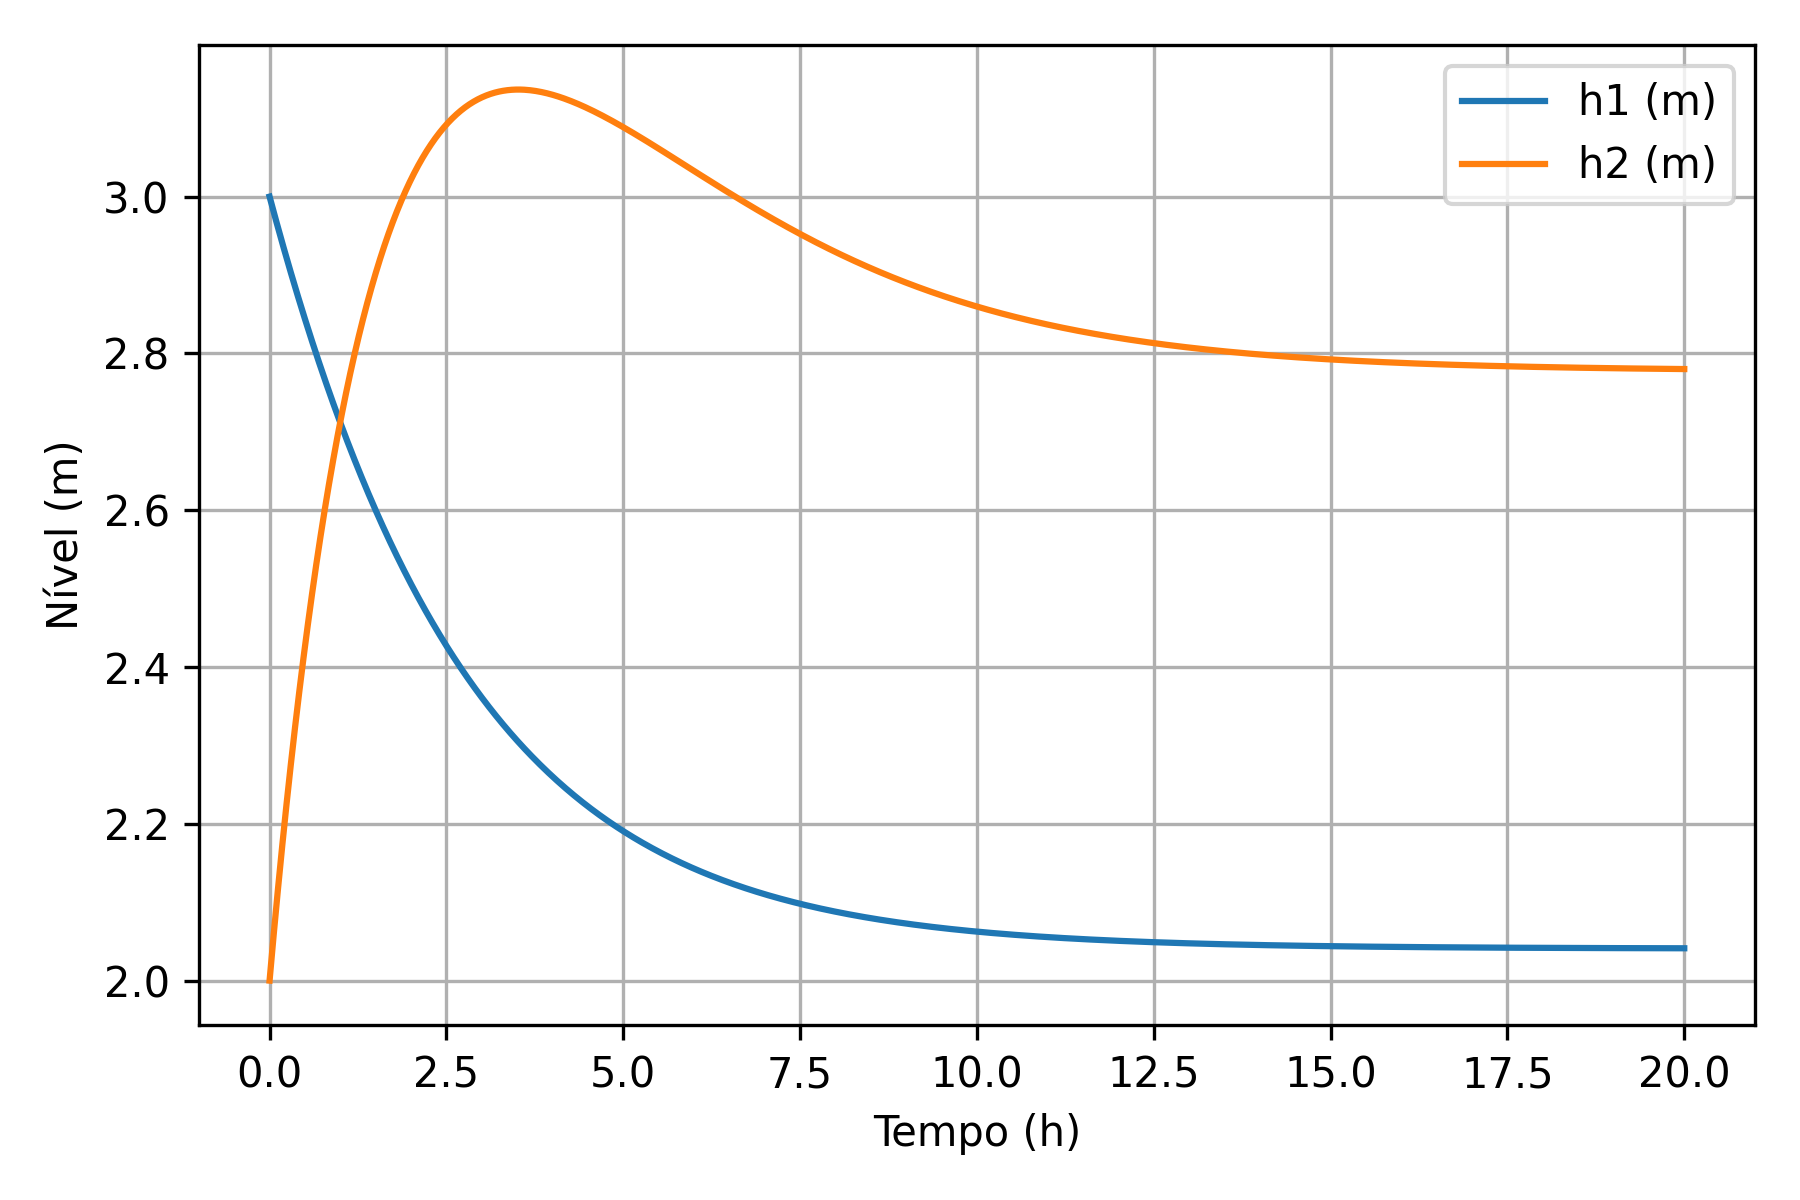
\includegraphics[width=0.7\textwidth]{figuras/questao1_niveis.png}
  \caption{Perfis temporais simulados dos níveis $h_1$ e $h_2$ durante 20 horas.}
  \label{fig:questao1}
\end{figure}
\begin{thebibliography}{9}
  \bibitem{referencia-exemplo}
  Autor, \emph{Título do Livro ou Artigo}, Editora, Ano.
\end{thebibliography}

\end{document}
